\subsection{Ergänzungen zum Zusammenspiel und Ablaufskizze}
In diesem Abschnitt wird der Ablauf des Programms skizziert. Dabei wird davon ausgegangen, dass KinectControl bereits instanziiert und durch Aufruf der \texttt{init()}-Funktion initialisiert wurde. Weiterhin gilt die Vorstellung, dass die \texttt{run()}-Methode im Main-Loop der umgebenden Software ausgeführt wird. Genaueres zur Einbindung ist Abschnitt \ref{sec:einbinden} zu entnehmen.\par 
Sollte kein Master bestimmt sein, so werden für den Master zunächst eindeutige Defaultwerte für ID (der negative Wert $-1$) und $z$"=Entfernung zur Kamera (der maximale Wert des Floatdatentyps) angenommen.\par 
Dann wird versucht, über den \texttt{BodyFrameReader} der Kinect einen aktuellen Kinect-Frame abzugreifen. Sollte dies fehlschlagen, so werden die alten Bewegungsparameter einfach weiterverwendet. Im Falle des Erfolgs wird versucht, auf die Körpertracking-Daten der Kinect zuzugreifen, was im Fehlerfall analog behandelt wird. Gerade die erste Art von Fehlschlag (der Versuch, einen Kinect-Frame zu holen, obwohl kein solcher vorhanden ist) tritt dabei tatsächlich häufig ein, da die Kinect nur etwa 30 Frames pro Sekunde liefern, wohingegen der Tick des Main Loops üblicherweise deutlich darüber liegt.\par 
Nachfolgend findet im Code die Masterbehandlung statt. Hier werden vier Fälle unterschieden, die gesondert erklärt werden sollen:
\begin{itemize}
%
\item Der weitere Programmablauf sei nun zunächst für den Fall geschildert, dass kein Master eingespeichert wird oder wurde. In diesem Falle ist der nächste relevante Schritt das Iterieren über die Körper, die die Kinect zurückgeliefert hat. Dabei werden die genauen Körperdaten abgefragt, namentlich die Positionen und Orientierungen der Gelenke. In der genannten Situation (vor jeglicher Masterfestlegung) wird als Basislösung der primitive $z$-Test zur Festlegung einer Person, die das Programm steuert, verwendet. Dazu wird das Master-Objekt einfach mit den Werten des Körpers belegt, dessen Kopf den niedrigsten $z$"=Wert aufweist. 
\item Das Programmverhalten ändert sich, wenn durch Betätigen der Einspeichertaste X ein Master festgelegt werden soll. Eine entsprechende Abfrage im Main-Loop des unterliegenden Programmes ruft die \texttt{assignMaster()}-Funktion von KinectControl auf, die die für die Masterfestlegung wichtigen Parameter initialisiert. Vor allem werden die booleschen Variablen \texttt{masterDetermined} und \texttt{collectFrames} auf \texttt{true} gesetzt und je nach Länge des Tastendrucks eine Variable hochgezählt, die die Anzahl der Samples für die Vermessung bestimmt. Fall zwei bei der Masterbehandlung entspricht dann der Belegung der beiden Variablen \texttt{masterDetermined} und \texttt{collectFrames} mit \texttt{true}. In diesem Falle wird beim Iterieren über die Körper zunächst ein Skelett in Standardpose gesucht. Die ID dieses Skeletts wird gespeichert und die zugehörige Person soll als Master eingespeichert werden. Befinden sich mehrere Skelette in Standardpose, so wird das indexmäßig erste im \texttt{trackedBodies}-Array für die Masterfestlegung verwendet. Nachdem die genannte ID und damit der künftige Master festgelegt ist, werden solange Körpermerkmale gesammelt, wie durch den Framezähler aus \texttt{assignMaster()} vorgegeben. Dazu wird die \texttt{collectBodyProperties()}-Funktion aus der \texttt{Person}-Klasse aufgerufen, die wie weiter oben ausgeführt ein festes Set an Körpermerkmalen puffert. Sollte der designierte Master dabei die Standardpose verlassen, wird die bisherige Sammlung mittels \texttt{deleteCollectedBodyProperties()} vollständig verworfen und die ID-Festlegung durch Standardposensuche vom Anfang erneut durchgeführt. War der Frame hingegen gut, wird die Anzahl noch zu sammelnder Frames dekrementiert. Sind genau so viele Frames gesammelt, wie durch \texttt{assignMaster()} vorgegeben wurde, so wird die Masterfestlegung durch Rücksetzen von \texttt{collectFrames} auf \texttt{false} und Aufruf von \texttt{calculateBodyProperties()} (ebenfalls aus der \texttt{Person}-Klasse) beendet. Konzeptuell erstellt letztere Funktion aus den vorher gesammelten Daten einen charakteristischen Vektor für die eingespeicherte Person, den sie im Master-Objekt ablegt.
\item Der dritte Fall in Sachen Masterfestlegung schließt sich sodann an, wenn also ein Master bestimmt wurde (\texttt{masterDetermined} ist \texttt{true}), jedoch keine Samples mehr gesammelt werden müssen (\texttt{collectFrames} ist \texttt{false}), weil der charakteristischen Vektor bereits gebildet wurde und verwendet werden kann. Dann muss hinsichtlich des Masters nur noch etwas getan werden, falls der Master zwischenzeitlich aus dem Tracking verschwunden ist, was vor der Iteration über die Körper überprüft wird. In diesem Falle wird \texttt{searchForMaster} gesetzt. Für die 0-1-Flanke von \texttt{searchForMaster} wird ein spezielles \texttt{lostMaster}-Flag gesetzt. In der Iteration über die Körper wird dann nach Körpern in Standardpose Ausschau gehalten und für diese Körper eine Sammlung von Abweichungswerten zum charakteristischen Vektor des Masters aufgebaut. Auf Codeebene wird dies durch ein Array von Puffern, \texttt{deviationBuffer[]}, gelöst. Die Abweichungen werden durch Aufruf der \texttt{compareBodyProperties()}-Methode der \texttt{Person}-Klasse berechnet. Das korrekte Weitersammeln in einem angefangenen Puffer kann über die von der Kinect vergebene, eindeutige \texttt{trackingId} gesichert werden. Die Puffer haben eine feste Größe und werden, wenn sie voll -- aktuell entspricht dies 20 Samples -- sind, durch Aufruf von \texttt{evaluateDeviationBuffer()} gemittelt. Ergebnis ist ein gemittelter Abweichungswert vom charakteristischen Vektor des Masters. Unterschreitet dieser eine empirisch festgelegte Grenze, lautet die Annahme, dass die präsentierte Person der Master ist und setzen das \texttt{master}-Objekt der Zustandsmaschine entsprechend.\par 
\item Als letzter Punkt in Sachen Masterbehandlung ist noch das Verhalten im Falle eines Masterverlusts (\texttt{lostMaster} ist dann \texttt{true}) zu klären. In diesem Falle werden sämtliche Bewegungsparameter und der Zustand der State-Machine zurückgesetzt. Außerdem wird \texttt{lostMaster} wieder auf \texttt{false} gesetzt, was den Effekt hat, dass die Variable tatsächlich genau die 0-1-Flanke von \texttt{searchForMaster} einfängt.\par
\end{itemize}
Im Programmtext und Ablauf folgt nach der Masterbehandlungsphase nun die Masterauslesung zur Steuerung des Programms. Sie findet statt, falls ein aktiver Master vorhanden ist. Von diesem werden sodann die Gelenke mit ihren Orientierungen und die Status der Hände ausgelesen. Die entsprechenden und wichtigen Merkmale werden im \texttt{master}-Objekt (z.\,T. nach Plausibilitätsüberprüfungen und gepuffert) abgelegt. Dann findet die Kernberechnung der Zustandsmaschine statt (siehe Abb. \ref{fig:ber}). In \texttt{bufferGestureConfidence()} wird aus den Joints und HandStates unter Verwendung eines Puffers ein Konfidenzvektor für die Gesten erstellt. In \texttt{compute()} findet die Berechnung der \texttt{motionParameters} entsprechend des aktuellen Zustands und der Gelenkdaten statt. Die Funktion \texttt{switchState()} nimmt schließlich anhand des Gestenkonfidenzvektors gegebenenfalls einen Zustandsübergang vor. Konzeptuelle Erläuterungen zur Funktionsweise dieser Funktionen sind in den vorangegangenen Abschnitten zu finden.\par\medskip
\begin{figure}[h]
\centering
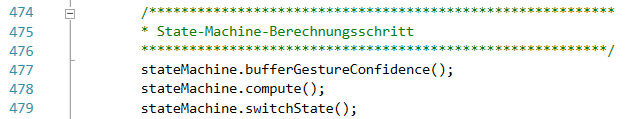
\includegraphics[width=.8\textwidth]{pictures/statemachine-ber.png}
\caption{Der Code, der den Berechnungsschritt der State-Machine darstellt.}\label{fig:ber}
\end{figure}
Am Ende der \texttt{run()}-Methode wird der Frame freigegeben und die bei \texttt{compute()} berechneten \texttt{motionParameters} zurückgegeben. Wie genau sie schließlich verwendet werden, entscheidet das unterliegende Programm.
